% Don't modify this section unless you know what you're doing!
\documentclass[letterpaper,12pt]{article}
\usepackage{float}
\usepackage[spanish]{babel}
\selectlanguage{spanish}
\usepackage[utf8]{inputenc}
\usepackage{tabularx} % extra features for tabular environment
\usepackage{amsmath}  % improve math presentation
\usepackage{graphicx, wrapfig, subcaption, setspace, booktabs}
\usepackage{graphicx} % takes care of graphic including machinery

\usepackage[margin=1in,letterpaper]{geometry} % decreases margins
\usepackage{cite} % takes care of citations
\usepackage[final]{hyperref} % adds hyper links inside the generated pdf file
\usepackage{amsmath}
\usepackage{amssymb}
\usepackage{enumerate}
\usepackage{url}
\hypersetup{
	colorlinks=true,       % false: boxed links; true: colored links
	linkcolor=blue,        % color of internal links
	citecolor=blue,        % color of links to bibliography
	filecolor=magenta,     % color of file links
	urlcolor=blue         
}
%++++++++++++++++++++++++++++++++++++++++


\begin{document}

\title{Reporte de la actividad 8}
\author{Daniela Olmos Velderrain\\Grupo 3}
\date{08 de abril de 2019}

\maketitle

\section{Introducción}
En esta actividad se trabajó sobre dos archivos de datos tomados de la estación de un Nogal. Tales datos corresponden a las temperaturas del suelo y del aire durante el año 2009. 
\\
\\
El objetivo fue unir dos diferentes conjuntos de datos mediante una variable temporal en común, y así estudiar las temperaturas del suelo a profundidades distintas, al igual que la temperatura del aire.
    
    
\section{Desarrollo}
\subsection{Metodología} 
Para trabajar con ambos archivos, fue necesario descargar ciertas librerías para el análisis de datos y visualización, así como para cálculos matemáticos y para poder trabajar en formato de fecha:

\begin{verbatim}
import pandas as pd
import numpy as np
import matplotlib.pyplot as plt
import seaborn as sns
import math
import datetime
\end{verbatim}

Se leyó el primer archivo con los datos meteorológicos de la estación del nogal:

\begin{verbatim}
    df1 = pd.DataFrame( pd.read_csv("meteo-nogal-09.csv", engine="python" ) )
\end{verbatim}

Este archivo ya se trabajó anteriormente en la Actividad 7, por lo que fueron seguidos los mismos pasos, pero esta vez creando un formato de fecha, ya que ambos archivos se unirán mediante esta variable.
\\
\\
Se siguió con la lectura del segundo archivo que contenía los datos de la tierra en la misma plantación de nogal:

\begin{verbatim}
    df2 = pd.DataFrame( pd.read_csv("soil-nogal-09.csv", engine="python" ) )
\end{verbatim}

Se filtraron las columnas de interés con datos correspondientes a fechas y temperaturas del suelo a distintas profundidades:

\begin{verbatim}
    df2 = df2.filter(['2 Year_RTM  L','3 Day_RTM  L','4 Hour_Minute_RTM  L',
    'Tsuelo_10cm','Tsuelo_20cm','Tsuelo_30cm','Tsuelo_40cm','Tsuelo_55cm',
    'Tsuelo_70cm','Tsuelo_85cm','Tsuelo_100cm'],axis=1)
\end{verbatim}

Dado que en el segundo archivo las horas y los minutos se encuentran mezclados en el formato, se crearon dos arreglos para separarlos. Primero, se convirtió la columna de horas y minutos a tipo string:

\begin{verbatim}
    df2['4 Hour_Minute_RTM  L'] = df2['4 Hour_Minute_RTM  L'].astype(str)
\end{verbatim}

Después, se extrajeron de dicha columna las horas y los minutos por separado y se acomodaron en los arreglos correspondientes:

\begin{verbatim}
hora=[]
minuto=[]

for i in range (0, len(df2)):
    #Primero revisaremos si contiene 4 caracteres.
    if (len(str(df2['4 Hour_Minute_RTM  L'][i]))==4):
        #Si resulta ser de 4 caracteres, revisaremos el caso en que la hora sea 2400.
        if (str(df2['4 Hour_Minute_RTM  L'][i])[0:2]=='24'):
            hora.append('00')
            minuto.append('00')
        else:
            hora.append(str(df2['4 Hour_Minute_RTM  L'][i])[0:2])
            minuto.append(str(df2['4 Hour_Minute_RTM  L'][i])[2:4])
    #Ahora revisamos el caso de que contenga 3 caracteres.
    elif (len(str(df2['4 Hour_Minute_RTM  L'][i]))==3):
            hora.append(str(df2['4 Hour_Minute_RTM  L'][i])[0:1])
            minuto.append(str(df2['4 Hour_Minute_RTM  L'][i])[1:3])
    #Por último revisaremos el caso de 2 caracteres.
    elif (len(str(df2['4 Hour_Minute_RTM  L'][i]))==2):
            hora.append('00')
            minuto.append(str(df2['4 Hour_Minute_RTM  L'][i])[0:2])

\end{verbatim}

A continuación, se creó un arreglo para almacenar los días:

\begin{verbatim}
    dias =[df2['3 Day_RTM  L'][i] for i in range(0,len(df2))]
\end{verbatim}

Posteriormente, se creó un data frame con los días, las horas y los minutos:

\begin{verbatim}
    d = {'dias': dias, 'hora': hora, 'minuto':minuto}
    df_fechas = pd.DataFrame(data=d)
\end{verbatim}

Dado que en este archivo la hora "00:00:00" se marca como un día anterior, se creó una nueva columna de días donde se aumenta un día cuando el reloj marque tal hora.  

\begin{verbatim}
dia=[]
for i in range(0,len(df_fechas)):
    if (df_fechas['hora'][i]=='00' and df_fechas['minuto'][i]=='00'):
        dia.append(df_fechas['dias'][i] +1)
    else:
        dia.append(df_fechas['dias'][i])
df_fechas['dia']=dia
\end{verbatim}

Ya con los días corregidos, se crea un arreglo de fechas de tipo string, con el año, los días, horas y minutos separados por espacios:

\begin{verbatim}
fechas = []
for i in range (0,len(df2)):
    fechas.append('2009 '+str(df_fechas['dia'][i])
    + ' ' + df_fechas['hora'][i]+' '+df_fechas['minuto'][i])

\end{verbatim}

A continuación, se tomó este arreglo y se le dio formato de fecha, tomando en cuenta que los días se encuentran escritos en un formato distinto al requerido:

\begin{verbatim}
FECHA = []
for i in range(0,len(df2)):
    d=datetime.datetime.strptime(fechas[i],'%Y %j %H %M')
    F = d.isoformat(' ')
    FECHA.append(F)
df2['FECHAN']=FECHA    
\end{verbatim}

Dado que los dos data frames trabajados tienen datos duplicados por fecha, estos fueron eliminados de ambos:

\begin{verbatim}
    df1 = df1.drop_duplicates(subset=['FECHA'])
    df2 = df2.drop_duplicates(subset=['FECHA'])
\end{verbatim}

Una vez filtrados los datos, se unieron ambos data frames mediante la función "merge", acomodando los datos de acuerdo a la columna de fecha creada:

\begin{verbatim}
    df3 = pd.merge(df1, df2, on=['FECHA'])
\end{verbatim}

A partir de este nuevo data frame se realizaron las gráficas requeridas, tomando datos para el periodo de tiempo solicitado, y utilizando las funciones \emph{groupby} y \emph{transform}.
\\
Después, se elaboraron las mismas gráficas, utilizando ahora el concepto de \emph{rolling mean} o \emph{promedio móvil}. 

\subsection{Resultados}
A continuación se muestran las gráficas elaboradas con Seaborn:

\begin{center}
	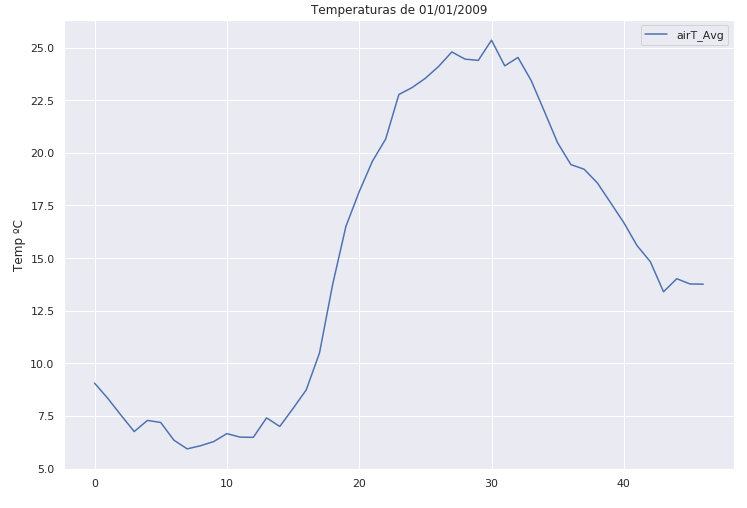
\includegraphics[height=5cm]{Tairundia.png}\hspace*{\fill}
	\label{graf1}
   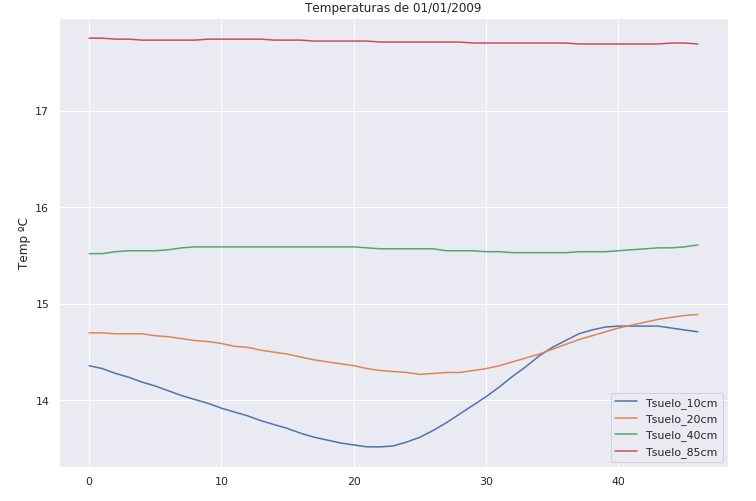
\includegraphics[height=5cm]{Tsueloundia.png}
    \label{graf2}
\end{center}

En estas dos gráficas se muestran 4 diferentes temperaturas del suelo y la temperatura del aire para el 1 de enero del 2009. 
\\
\\
\begin{center}
	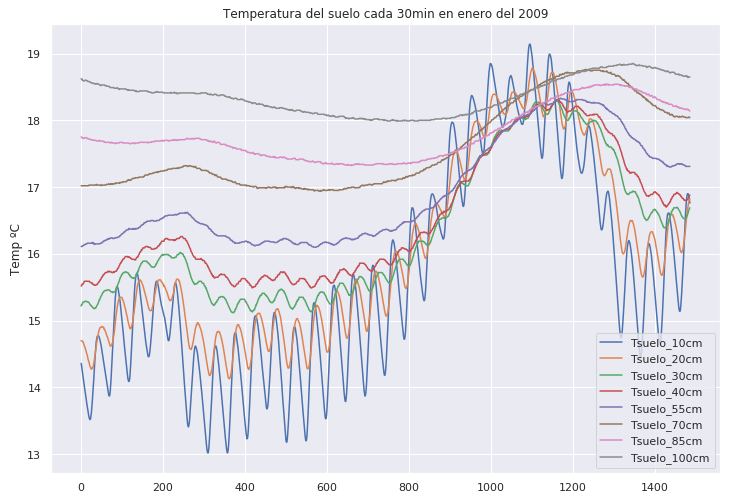
\includegraphics[height=5cm]{T30SueloEnero.png}\hspace*{\fill}
	\label{graf3}
   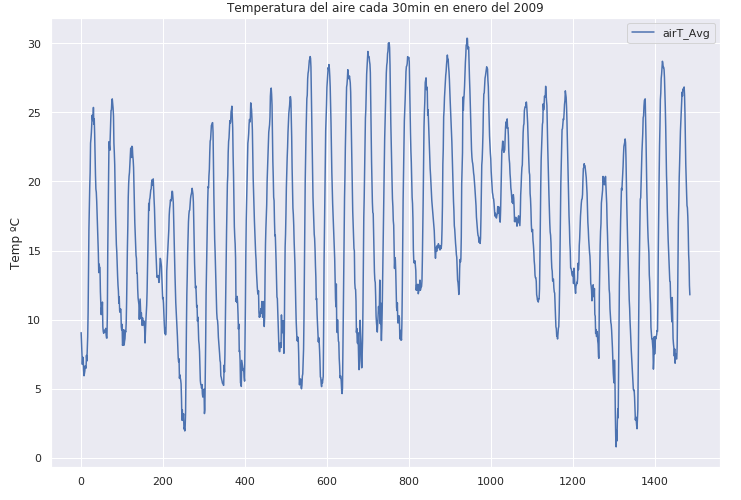
\includegraphics[height=5cm]{T30AireEnero.png}
    \label{graf4}
\end{center}

En el par de gráficas mostradas se aprecian las temperaturas del suelo y del aire para enero del 2009.
\\
\\
En las gráficas siguientes se pueden ver las temperaturas máximas, mínimas y promedio del aire y del suelo a diferentes profundidades para cada día de 2009. Se realizó una comparación para cada gráfica con su gráfica realizada mediante el promedio móvil.

\begin{center}
	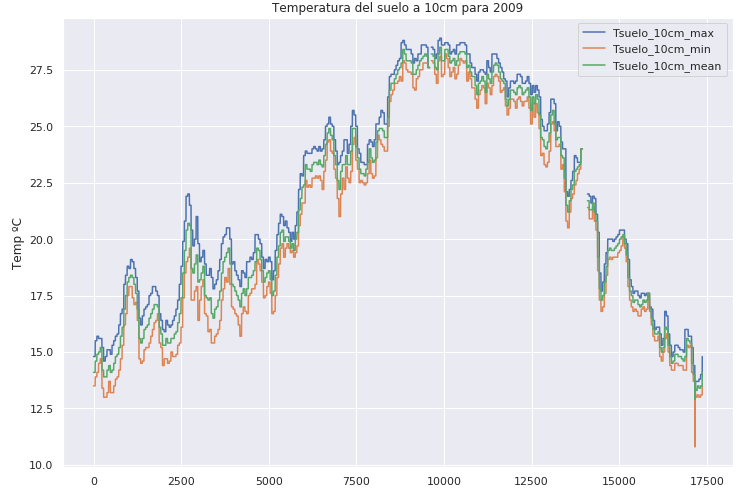
\includegraphics[height=5cm]{T10.png}\hspace*{\fill}
	\label{graf5}
   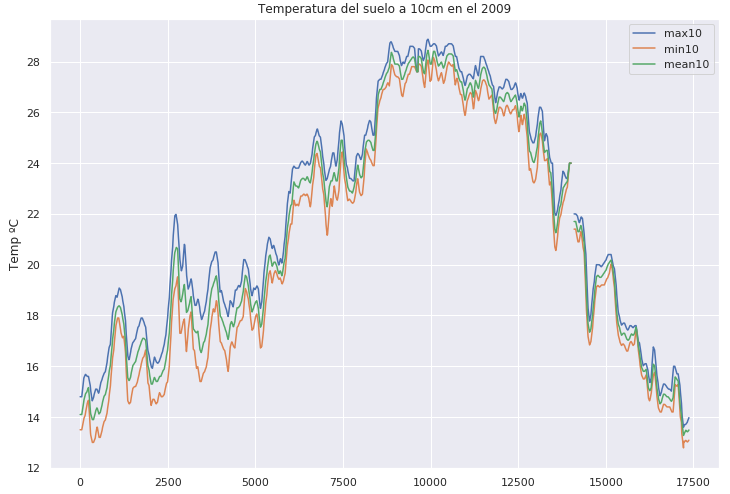
\includegraphics[height=5cm]{T10roll.png}
    \label{graf6}
\end{center}

\begin{center}
	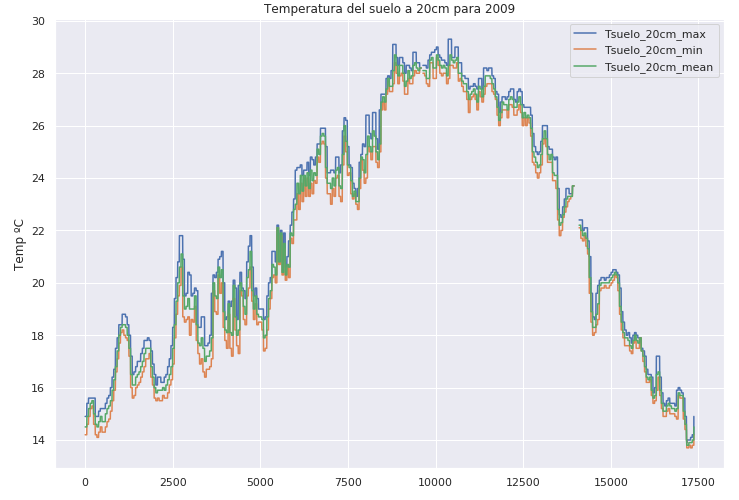
\includegraphics[height=5cm]{T20.png}\hspace*{\fill}
	\label{graf7}
   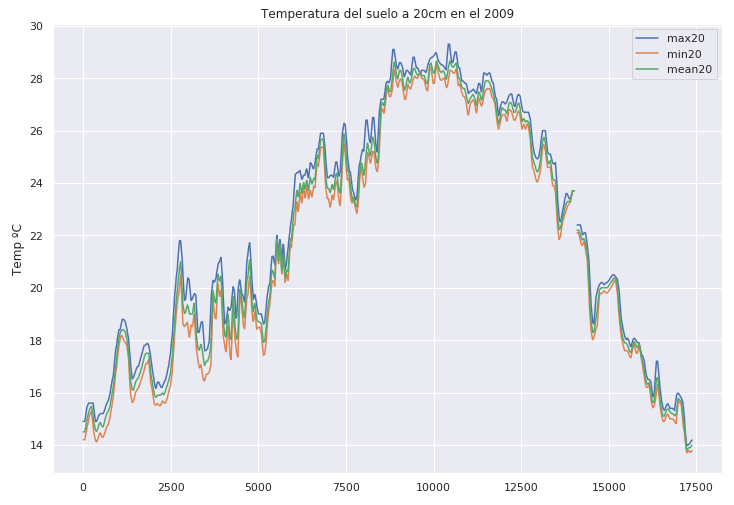
\includegraphics[height=5cm]{T20roll.png}
    \label{graf8}
\end{center}

\begin{center}
	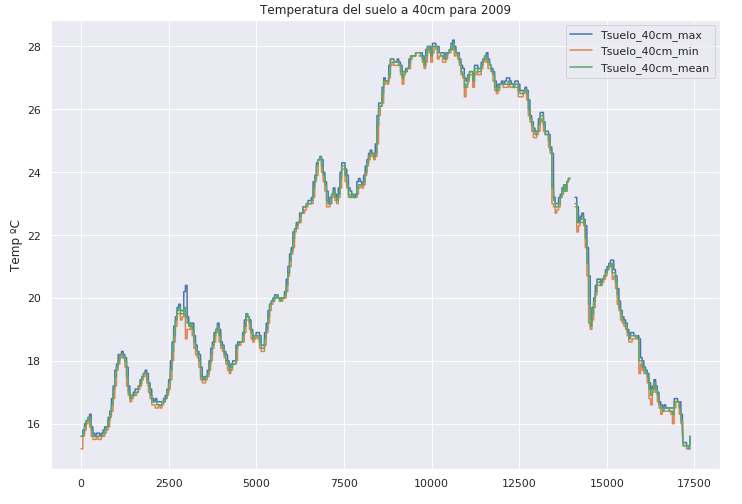
\includegraphics[height=5cm]{T40.png}\hspace*{\fill}
	\label{graf9}
   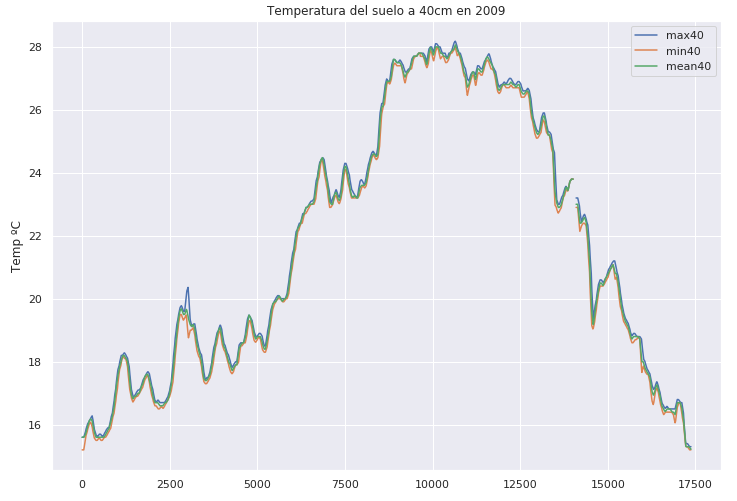
\includegraphics[height=5cm]{T40roll.png}
    \label{graf10}
\end{center}

\begin{center}
	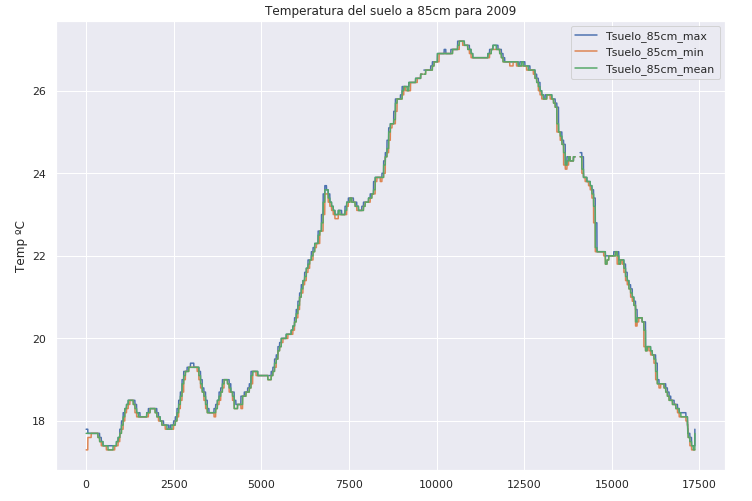
\includegraphics[height=5cm]{T85.png}\hspace*{\fill}
	\label{graf11}
   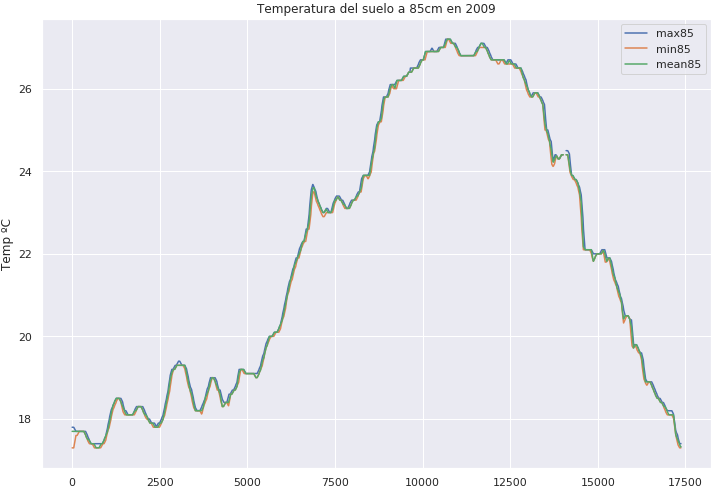
\includegraphics[height=5cm]{T85roll.png}
    \label{graf12}
\end{center}

\section{Conclusiones}

En las gráficas para el 1 de enero del 2009 se puede apreciar que la temperatura del subsuelo varía más mientras más cerca de la superficie se tome la medición. A mayor profundidad, la temperatura es mayor y presenta menos variaciones. En contraste, la temperatura del aire tiene marcadas diferencias entre su valor máximo y mínimo a través del día. 
\\
\\
Esto también se puede apreciar en las gráficas para el promedio cada 30 minutos, donde las temperaturas más profundas del subsuelo son las más estables y cálidas.
\\
\\
En las gráficas de temperatura máxima, mínima y promedio se observa con mayor claridad la conclusión de las gráficas anteriores. Mientras más profundo se tome la medición de temperatura, más parecidas son sus gráficas de valores máximo, mínimo y promedio. En el caso de la gráfica para la temperatura del aire, esta tiene la diferencia de valores más marcada. 
\\
\\
Cabe destacar también el uso del promedio móvil, ya que ayudó a suavizar las gráficas, dando una mejor idea de la tendencia que siguen los datos.
\\
\\
Como comentario final, en esta actividad la mayor dificultad se encontró en unir dos conjuntos de datos en uno solo, lo cual será de mucha utilidad para trabajos futuros.    

\section*{Bibliografía}
\begin{itemize}

\item \\Python Strings, Functions and Examples. Recuperado el 8 de abril de 2019 desde \\https://www.techbeamers.com/python-strings-functions-and-examples/
\\

\item \\Merge, join and concatenate. Recuperado el 8 de abril de 2019 desde \\https://pandas.pydata.org/pandas-docs/stable/user\_guide/merging.html
\end{itemize}


\end{document}
